\section{Materials and Methods}
\label{sec:methods}

\subsection{Experimental Design}
\label{subsec:design}

Three arms choose the training hyperparameters of the same detector (Fig.~\ref{fig:pipeline}). \armA uses the Ultralytics defaults with no search, and is the reference that any tuning has to beat. \armB takes the best of 32 random samples. \armC takes the best setting found by a swarm of 8 particles over 4 rounds. Both search arms score their candidates with the same proxy training (Section~\ref{subsec:proxy}). The budget is therefore counted in proxy trainings and not in wall-clock time, which varied between methods and cloud sessions (Section~\ref{subsec:res-cost}). The setting chosen by each arm is trained once with the same recipe (Section~\ref{subsec:training}) and scored once on a held-out test split (Section~\ref{subsec:eval}).

We ran the experiment twice. \genone uses one studio-style dataset with six classes at 416~px. \gentwo adds real-world training photographs, a seventh class (OTHER), 640~px images and an Indian set used only for testing. The search space, PSO settings, seeds, training recipe and evaluation code are the same in both, and both searches were run again from scratch for \gentwo. Because the classes, image size and training data differ, scores from the two generations cannot be compared directly. Section~\ref{subsec:eval} describes a separate comparison on common test images.

\begin{figure}[!t]
\centering
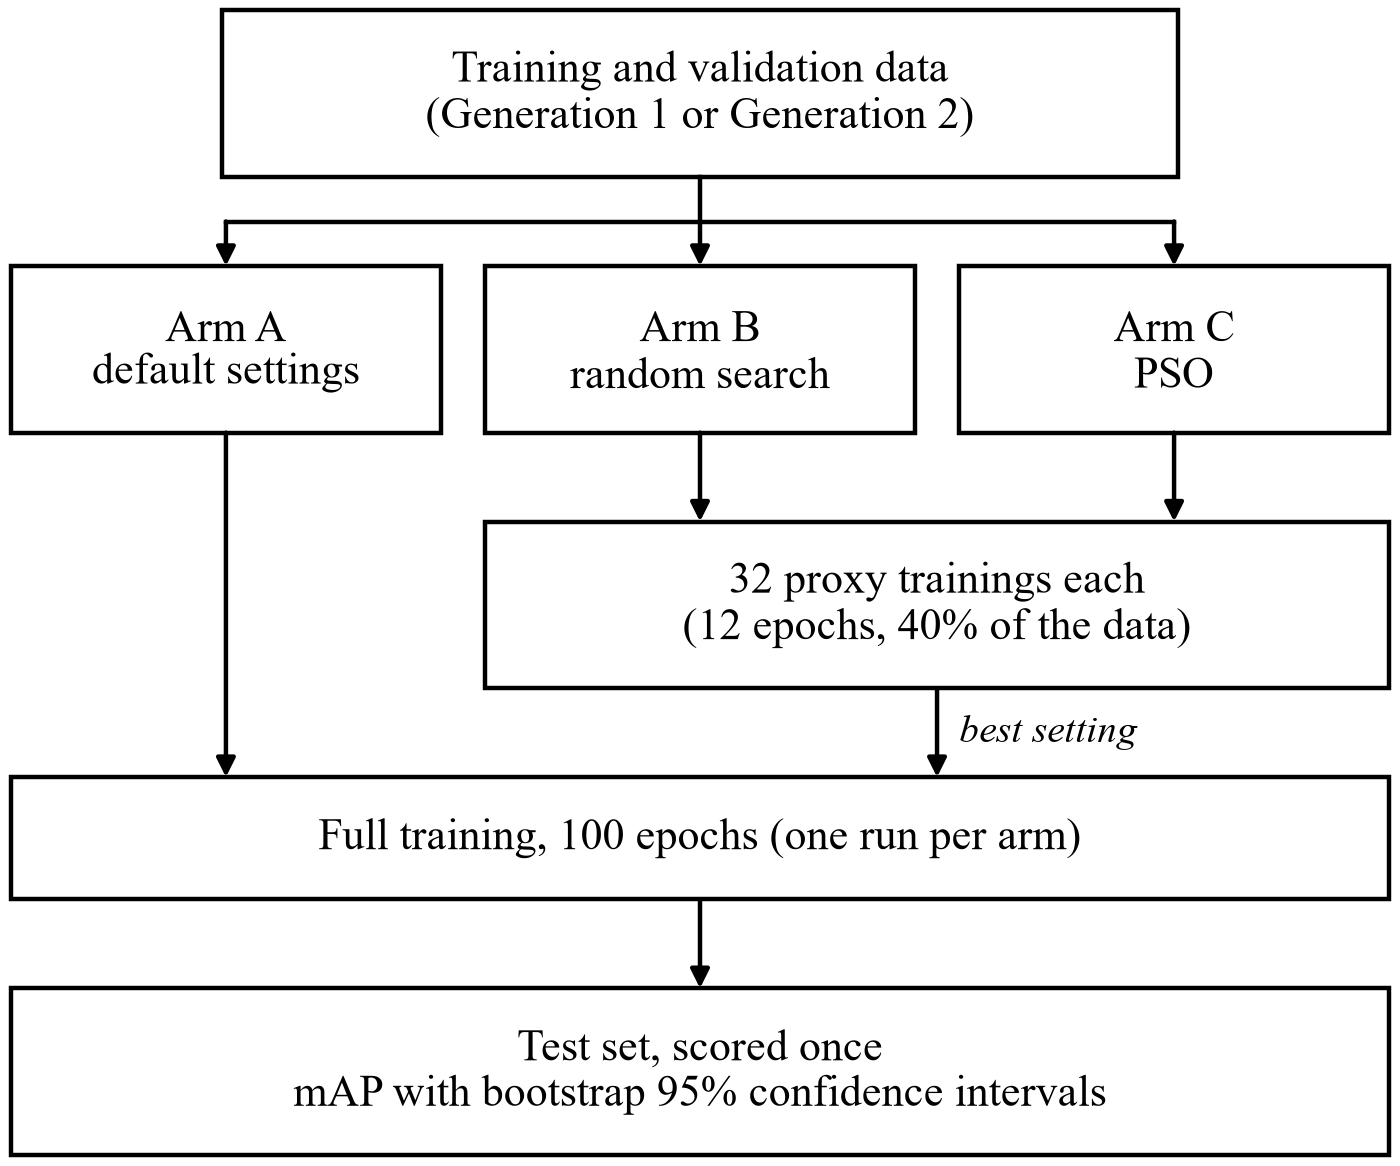
\includegraphics[width=\columnwidth]{m_pipeline.png}
\caption{Experimental pipeline, the same in both generations. Arms~B and~C each spend 32 proxy trainings, and Arm~A uses the library defaults without a search.}
\label{fig:pipeline}
\end{figure}

\subsection{Datasets}
\label{subsec:datasets}

Table~\ref{tab:datasets} lists the sources with their licences and split sizes.

\textit{\genone data.} The Kaggle dataset ``Garbage Detection -- 6 Waste Categories''~\cite{viswaprakash2024garbage}, exported from a Roboflow project, contains studio-style images with YOLO boxes in six classes: BIODEGRADABLE, CARDBOARD, GLASS, METAL, PAPER and PLASTIC. The data are imbalanced. In the training split, BIODEGRADABLE has 61.92\% of the boxes and PAPER 5.61\%, and 36.45\% of the boxes cover less than 1\% of the image. The folders that come with the dataset are split by class in an unusable way (the validation folder has 13,632 BIODEGRADABLE boxes but 33 PAPER boxes, and the test folder has no GLASS box). We therefore pooled all images and split them again 70/20/10, stratified by source class with seed 42, requiring at least 30 boxes per class in validation and test. Near-duplicate images were kept in the same split. Two images count as duplicates if the files are identical (MD5), if they come from the same Roboflow source image, or if their 256-bit difference hashes are within 10 bits, or within 40 bits with a Pearson correlation of at least 0.90 between $64\times64$ grayscale thumbnails. This gave 47 groups with 133 images. The label check found 17 zero-size boxes and no corrupt or unlabeled image.

\textit{\gentwo training data.} \gentwo has seven classes: the six \genone classes with the same indices, plus OTHER. From the \genone splits we kept a subsample of 3,000 training and 900 validation images, stratified by dominant class (seed 42), and all test images, so the \gentwo studio test set is the \genone test set. TACO~\cite{proenca2020taco} adds crowd-sourced photographs of litter in the wild. We mapped all 60 of its categories to our classes (drink cans to METAL and cigarettes to OTHER, for example), which gave 1,260 OTHER boxes but only 8 BIODEGRADABLE boxes. The HITL Recycling dataset~\cite{hitl2026recycling} adds street photographs, almost all with one litter box. We assigned its class from the object tag where that was decisive (food waste $\to$ BIODEGRADABLE), otherwise from the material tag (aluminum $\to$ METAL), and otherwise OTHER; 100 objects had no material tag. TACO and HITL were split 70/20/10 with the same duplicate rules and stored with a long side of at most 640~px. The merged data contain 962 duplicate groups, none of which spans two sources or two splits. Of these, 918 are byte-identical pairs inside the real-world sources. They cause no leakage but give some photographs extra weight. BIODEGRADABLE has 51.96\% of the training boxes and OTHER 3.89\%. The studio images contain no OTHER box, and the real-world test set contains a single BIODEGRADABLE box.

\textit{Indian test set.} DWSD~\cite{ali2025dwsd} has 784 phone photographs of streets, parks and garbage areas in Kolkata and Berhampore, West Bengal, annotated as $448\times448$ semantic masks. We used it only for testing, never for training, search or model selection. To get boxes, we turned each 8-connected region of one mask value (at least 50 pixels) into a box, which means that touching items of the same class end up in one large box. The class mapping had to be inferred. The published table of mask values does not match what the regions show (the value listed as background covers polythene bags in 610 masks), so we named each value by looking at its regions, and six of the fifteen values remain uncertain. We excluded the 84 images without boxes, because some of them show waste that is not annotated. This leaves 3,040 PLASTIC, 1,230 PAPER, 124 CARDBOARD, 90 OTHER and 18 METAL boxes. An MD5 check against the 9,647 images of the main build found no identical file.

\begin{table*}[!t]
\centering
\caption{Datasets. Counts are images, with boxes in parentheses. ``Classes'' is the number of target classes that occur in the source. The \gentwo studio test set equals the \genone test set; the \gentwo real-world test set is the union of the TACO and HITL test images (468 images, 779 boxes).}
\label{tab:datasets}
\footnotesize
\setlength{\tabcolsep}{4pt}
\begin{tabular}{@{}llllllccc@{}}
\toprule
Generation & Source & Domain & Licence & Stored size & Classes & Train & Validation & Test \\
\midrule
\genone & Garbage Detection (Kaggle) & studio & CC BY 4.0 & $416\times416$ & 6 & 7,324 (51,756) & 2,094 (14,904) & 1,046 (7,413) \\
\midrule
\multirow{5}{*}{\gentwo} & \genone subsample & studio & CC BY 4.0 & $416\times416$ & 6 & 3,000 (22,206) & 900 (6,904) & 1,046 (7,413) \\
 & TACO~\cite{proenca2020taco} & real-world & CC BY 4.0 & long side $\le 640$ & 7 & 1,050 (3,293) & 301 (1,031) & 149 (460) \\
 & HITL Recycling & real-world & CC0 & long side $\le 640$ & 7 & 2,242 (2,246) & 640 (641) & 319 (319) \\
 & Total (7 classes) & mixed & & & 7 & 6,292 (27,745) & 1,841 (8,576) & 1,514 (8,192) \\
 & DWSD~\cite{ali2025dwsd} & India & CC BY 4.0 & $448\times448$ & 5 & -- & -- & 700 (4,502) \\
\bottomrule
\end{tabular}
\end{table*}

\subsection{Detector}
\label{subsec:detector}

All arms train YOLOv8n, the nano model of the YOLOv8 single-stage detectors~\cite{redmon2016you,jocher2023ultralytics}, with Ultralytics 8.4.169. Training starts from COCO-pretrained weights~\cite{lin2014microsoft} with the class outputs resized to our six or seven classes. We chose the nano model because it can run on a smart bin or a phone, and because it makes 32 proxy trainings per arm affordable on one cloud GPU.

\subsection{Search Space}
\label{subsec:space}

Both search arms use the same six dimensions (Table~\ref{tab:space}): the initial learning rate \texttt{lr0}, the final learning rate as a fraction of the initial one (\texttt{lrf}), the SGD \texttt{momentum}, the \texttt{weight\_decay}, the probability of mosaic augmentation (\texttt{mosaic}) and the gain of random rescaling (\texttt{scale}). The optimizers work in what we call search units. \texttt{lr0} and \texttt{weight\_decay} span two orders of magnitude and are stored as base-10 exponents, so a particle at $-3.2$ means $\texttt{lr0}=10^{-3.2}$. The other four are stored as plain values. Decoded values are rounded to six significant digits. Three of the defaults lie on a boundary of the space (\texttt{lrf} on the lower bound, \texttt{lr0} and \texttt{mosaic} on the upper bounds), so the searches can reach them only at the edge. All other training hyperparameters keep the library defaults in every arm.

\begin{table}[!t]
\centering
\caption{Search Space and Search Settings (Shared by Both Generations)}
\label{tab:space}
\footnotesize
\begin{tabular}{@{}p{0.27\columnwidth}lll@{}}
\toprule
Hyperparameter & Range & Scale & Default (Arm~A) \\
\midrule
\texttt{lr0} & $10^{-4}$ to $10^{-2}$ & $\log_{10}$ & 0.01 \\
\texttt{lrf} & 0.01 to 0.2 & linear & 0.01 \\
\texttt{momentum} & 0.60 to 0.98 & linear & 0.937 \\
\texttt{weight\_decay} & $10^{-5}$ to $10^{-3}$ & $\log_{10}$ & 0.0005 \\
\texttt{mosaic} & 0.0 to 1.0 & linear & 1.0 \\
\texttt{scale} & 0.2 to 0.8 & linear & 0.5 \\
\midrule
Setting & \multicolumn{3}{l@{}}{Value} \\
\midrule
PSO budget & \multicolumn{3}{p{0.63\columnwidth}@{}}{8 particles $\times$ 4 rounds $=$ 32 evaluations} \\
Inertia $w_t$ & \multicolumn{3}{p{0.63\columnwidth}@{}}{0.9, 0.65, 0.4 (linear over 3 update steps)} \\
$c_1$, $c_2$ & \multicolumn{3}{p{0.63\columnwidth}@{}}{1.5, 1.5} \\
$\mathbf{r}_1$, $\mathbf{r}_2$ & \multicolumn{3}{p{0.63\columnwidth}@{}}{$U(0,1)$, fresh per particle and dimension} \\
Velocity limit & \multicolumn{3}{p{0.63\columnwidth}@{}}{$\pm20\%$ of each range} \\
Initialization & \multicolumn{3}{p{0.63\columnwidth}@{}}{positions uniform in bounds; velocities uniform in $\pm10\%$ of each range} \\
Boundaries & \multicolumn{3}{p{0.63\columnwidth}@{}}{position clipped; velocity of a clipped dimension set to 0} \\
PSO seed & \multicolumn{3}{p{0.63\columnwidth}@{}}{42} \\
Random search & \multicolumn{3}{p{0.63\columnwidth}@{}}{32 i.i.d.\ uniform samples in search units; seed 123} \\
Fitness & \multicolumn{3}{p{0.63\columnwidth}@{}}{validation \mapfifty after a 12-epoch proxy training on a stratified 40\% training subset} \\
\bottomrule
\end{tabular}
\end{table}

\subsection{Particle Swarm Optimization}
\label{subsec:pso}

Arm~C uses a global-best PSO~\cite{kennedy1995particle} with an inertia weight~\cite{shi1998modified}, which we wrote in NumPy. It maximizes the proxy fitness. Particle $i$ has a position $\mathbf{x}_i \in \mathbb{R}^6$ in search units, a velocity $\mathbf{v}_i$ and a personal best position $\mathbf{p}_i$, and $\mathbf{g}$ is the best position of the swarm. One update step is
\begin{equation}
\mathbf{v}_i \leftarrow w_t\,\mathbf{v}_i + c_1\,\mathbf{r}_1 \odot (\mathbf{p}_i - \mathbf{x}_i) + c_2\,\mathbf{r}_2 \odot (\mathbf{g} - \mathbf{x}_i),
\label{eq:velocity}
\end{equation}
where $\odot$ is the element-wise product and $\mathbf{r}_1$, $\mathbf{r}_2$ are drawn again at every step (Table~\ref{tab:space}). Each component $v_{i,d}$ is then clamped to $[-v_{\max,d},\, v_{\max,d}]$ with $v_{\max,d} = 0.2\,(u_d - l_d)$, where $l_d$ and $u_d$ are the bounds of dimension $d$, and the position is updated element-wise as
\begin{equation}
\mathbf{x}_i \leftarrow \min\bigl(\max(\mathbf{x}_i + \mathbf{v}_i,\ \mathbf{l}),\ \mathbf{u}\bigr).
\label{eq:position}
\end{equation}
If a dimension is clipped, its velocity is set to zero, so the particle stays at the wall. Round~1 evaluates the random initial swarm and each of the $T-1 = 3$ update steps is followed by one more round, so $T = 4$ rounds use exactly 32 evaluations. The inertia weight falls linearly,
\begin{equation}
w_t = w_{\mathrm{start}} - (w_{\mathrm{start}} - w_{\mathrm{end}})\,\frac{t-1}{T-2}, \qquad t = 1, \dots, T-1,
\label{eq:inertia}
\end{equation}
from $w_{\mathrm{start}} = 0.9$ to $w_{\mathrm{end}} = 0.4$. The inertia weight itself is from~\cite{shi1998modified}; the linear schedule is our own choice, so that the swarm explores first and refines later. A personal best is replaced only by a strictly higher fitness. All random numbers come from one seeded generator, which lets an interrupted search resume exactly by replaying the seed and the logged fitness values. A failed training (non-finite \mapfifty) would be given fitness 0, but none occurred in the four searches.

To check the code, we ran the optimizer with 20 particles, 50 rounds and 10 seeds on $[-5.12, 5.12]^6$. The median best value was $1.9\times10^{-5}$ on the Sphere function and 6.96 on the multimodal Rastrigin function (both have minimum 0), so the optimizer converges on a smooth function and still makes progress on one with many local minima.

\subsection{Random Search and Defaults}
\label{subsec:random}

Arm~B draws 32 points uniformly in search units, which is log-uniform for \texttt{lr0} and \texttt{weight\_decay}, and scores them with the same proxy and script as the swarm. We include random search~\cite{bergstra2012random} because a structured optimizer should beat it at the same budget. The winner of each search arm is the setting with the highest proxy fitness (the first one in case of a tie). Arm~A uses the defaults in Table~\ref{tab:space}.

\subsection{Proxy Fitness and Its Validation}
\label{subsec:proxy}

A full training takes more than an hour on our GPU, so the searches score candidates with a 12-epoch proxy training on a stratified 40\% subset of the training split: 2,930 of the 7,324 \genone images (stratified by source class) and 40\% of the 6,292 \gentwo images (by source and dominant class). The subset is drawn once with seed 42 and stored as an image list, so every candidate trains on the same images. The fitness is the validation \mapfifty of the last-epoch weights. The proxy follows the full-training recipe (Section~\ref{subsec:training}) with one change: the period without mosaic and the warm-up are shortened to keep their share of the run, 10\% and 3\% (\texttt{close\_mosaic} 1 epoch, warm-up 0.36 epochs). Otherwise the searched \texttt{mosaic} value would have a different effect in the proxy than in the full run.

Before the \genone searches we tested whether the proxy ranks settings like a longer training does. We drew seven configurations by Latin hypercube sampling~\cite{mckay1979comparison} in search units (SciPy, ``random-cd'', seed 42), added the defaults, and trained each one twice: with the proxy, and with a 40-epoch ``medium'' run on the full training split (\texttt{close\_mosaic} 4, warm-up 1.2 epochs), both at 416~px. The statistic was the Spearman rank correlation~\cite{spearman1904proof} of the eight score pairs. We fixed the pass threshold, $\rho \ge 0.6$, and the fallback, a 20-epoch proxy, before running the check. The result is in Section~\ref{subsec:res-proxy}.

We did not repeat the check for \gentwo. That decision was recorded before the \gentwo searches and relied on the \genone result and the unchanged recipe, so for the new data, classes and image size the validity of the proxy is assumed and not tested. The check is also small: eight configurations, a 40-epoch reference instead of 100 epochs, and last-epoch weights where the final models use \texttt{best.pt} (Section~\ref{subsec:limitations}).

\subsection{Full Training}
\label{subsec:training}

The setting chosen by each arm was trained once from the COCO-pretrained weights for 100 epochs on the full training split. The recipe was the same for the three arms: SGD, batch size 16, a 3-epoch warm-up, no mosaic in the last 10 epochs, and 416~px in \genone or 640~px in \gentwo. SGD had to be set explicitly, because the default \texttt{optimizer=auto} ignores the searched \texttt{lr0} and \texttt{momentum}; each run records the optimizer and learning rate it used. We tested the checkpoint with the best validation fitness (\texttt{best.pt}). All other arguments kept their defaults.

Every run used seed 42 in deterministic mode. Early on, the first training in a process gave different results from later ones. The cause was a module that Ultralytics imports lazily during the first training and that draws random numbers after seeding. Importing it before seeding removed the difference. All trainings ran on one NVIDIA Tesla T4 GPU on Kaggle with one training seed per arm, so we did not measure run-to-run variance (Section~\ref{subsec:limitations}).

Two \gentwo runs froze, most likely because the data mount of the session stopped responding. We resumed the Arm~C training from its epoch-55 checkpoint after checking every saved training argument against the plan. This continues the same weights, optimizer state and epoch counter, but it is not bit-identical to an uninterrupted run. The random search stopped after 11 of 32 evaluations and was continued by replaying its log, which does not affect the completed evaluations.

\subsection{Evaluation Protocol}
\label{subsec:eval}

Each test split was scored once, after all training was finished. Anything we needed to check earlier was checked on the validation split. In \gentwo, one run scored the three models on the whole test split (``all'', 1,514 images) and separately on the studio, real-world and India sets. Before scoring, each checkpoint had to match the record of its arm (classes, epochs, image size and the six hyperparameters).

We used the Ultralytics validator at each model's training image size (batch 32, rectangular batching, confidence threshold 0.001, NMS IoU 0.7, 32-bit floats). We report \mapfifty, \mapfiftyninetyfive (IoU 0.50 to 0.95 in steps of 0.05), precision and recall at the confidence of maximum F1, and per-class AP@50. As a check, we recomputed both mAP values from the stored per-image statistics. They had to match the validator within $10^{-4}$ and in fact agreed exactly.

Uncertainty is estimated with a paired image bootstrap~\cite{efron1993introduction}: 1,000 resamples of the test images (seed 0), using the same resampled indices for every model. We report 95\% percentile intervals for each model and for each pairwise difference, and call a difference significant only if its interval excludes 0. Each \gentwo test set has its own bootstrap. We computed no $p$-values and applied no multiple-comparison correction, per-class AP has no interval, and the intervals cover test sampling only, not training or search randomness.

To compare the two generations on the same images, we scored all six final models (three arms per generation) on the studio and real-world test sets, each at its own training image size, with the labels restricted to the six shared classes. OTHER labels were removed (images left empty stay in the set), and OTHER predictions of the \gentwo models were dropped in non-maximum suppression. The results are in Section~\ref{subsec:res-domain} and Table~\ref{tab:g1g2}.

Inference speed is the median batch-1 latency over 100 test images after 10 warm-up predictions (confidence 0.25) at the training image size. It was measured on a laptop CPU (Intel Core Ultra~5 125H) for \genone and on the T4 GPU for \gentwo, so it can be compared only within a generation.
